%&preamble
% automatic hyphenation for 2 languages
% http://www.mechpedia.gr/wiki/Hyphenation_-_%CE%A5%CF%86%CE%B5%CE%BD%CF%8E%CF%83%CE%B5%CE%B9%CF%82#.CE.91.CF.85.CF.84.CF.8C.CE.BC.CE.B1.CF.84.CE.B5.CF.82_.CF.85.CF.86.CE.B5.CE.BD.CF.8E.CF.83.CE.B5.CE.B9.CF.82_.CF.83.CE.B5_.CE.B4.CE.AF.CE.B3.CE.BB.CF.89.CF.83.CF.83.CE.B1_.CE.BA.CE.B5.CE.AF.CE.BC.CE.B5.CE.BD.CE.B1
% very slow, enable only at final pdf.
%\usepackage[Greek,Latin]{ucharclasses}
%\setTransitionsForGreek{\selectlanguage{greek}}{\selectlanguage{english}}

% polyglossia
\usepackage{polyglossia}
\setmainlanguage{greek}
\setotherlanguages{english}

% Fonts
% fonts can't go in the .fmt file
\usepackage{fontspec}
\setmainfont[Mapping=tex-text]{DejaVu Sans}
\newfontfamily\greekfont[Script=Greek]{DejaVu Sans}
\newfontfamily\greekfontsf[Script=Greek]{DejaVu Sans}
\setmonofont{Hack}
\newfontfamily\greekfonttt[Scale=1.0]{Hack}
\usepackage{microtype} % microtype is font-dependant


\title{%
  \vspace{0.3cm}%
  \hrule height 2pt%
  \vspace{0.3cm} Δίκτυα Υπολογιστών ΙΙ\\
  Εργασία Δικτυακού Προγραμματισμού%
  \vspace{0.3cm}%
  \hrule height 2pt%
  \vspace{0.3cm}
}

\author{%
  Φλώρος-Μαλιβίτσης Ορέστης, 7796  \href{mailto:orestisf@ece.auth.gr}{orestisf@ece.auth.gr}\\
  \textbf{Τομέας Ηλεκτρονικής}\\
  \textbf{Τμήμα Ηλ. Μηχανικών / Μηχανικών ΗΥ}\\
  \textbf{Αριστοτέλειο Πανεπιστήμιο Θεσσαλονίκης}
}
\titlepic{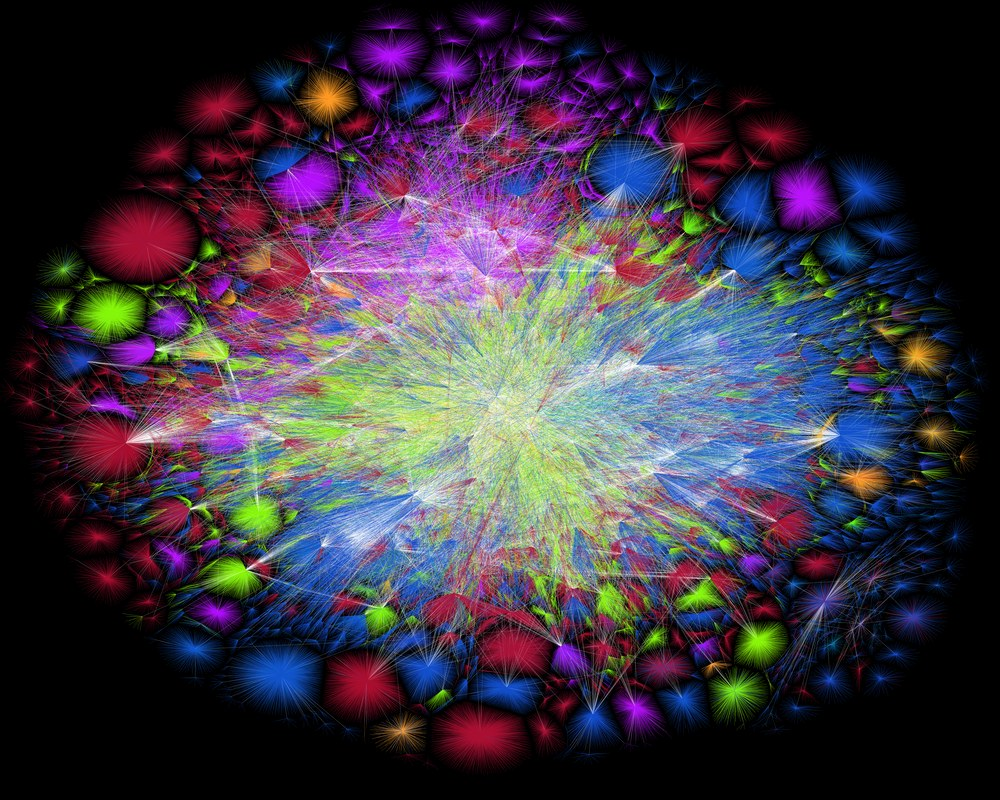
\includegraphics[width=0.70\textwidth]{images/cover}}

% Variables & constants definitions:
\newcommand{\appname}{\texttt{userApplication}}

\begin{document}
\pagenumbering{roman}
\deactivateBG
\maketitle
\tableofcontents
\listoflistings
\listoffigures
\listoftables
\clearpage % Ensure background starts after this.
% Chapters start from here on:
\activateBG
\pagenumbering{arabic}
\setcounter{page}{1}

\section{Εισαγωγή}
Αφορά την \sessionnumber{} σύνοδο με την Ιθάκη.
Η σύνοδος αυτή άρχισε στις \sessiondatestart{} και τελείωσε στις \sessiondateend{}.
Οι παράμετροι που χρησιμοποιήθηκαν φαίνονται στον πίνακα
\hyperref[table:codes]{\ref{table:codes}}.

\begin{table}
\centering
\begin{tabular}{c|c}
\hline
\multicolumn{1}{c}{\bfseries Παράμετρος} & \multicolumn{1}{|c}{\bfseries Τιμή}\\\hline
Client Address&\clientaddress{}\\
Client Listening Port&\clientlisteningport{}\\
Server Listening Port&\serverlisteningport{}\\
Echo Request Code&\echorequestcode{}\\
Image Request Code&\imagerequestcode{}\\
Sound Request Code&\soundrequestcode{}\\
\end{tabular}
\caption{Παράμετροι για την \sessionnumber{} σύνοδο}
\label{table:codes}
\end{table}
\FloatBarrier

\chapter{Βιβλιογραφική αναφορά}
\section{Το πρωτόκολλο UDP}
Το πρωτόκολλο UDP (User Datagram Protocol ή Universal Datagram Protocol)
είναι ένα από τα βασικά πρωτόκολλα που χρησιμοποιούνται στο Internet.
Σχεδιάστηκε το 1980 και ορίζεται στο RFC 768\cite{rfc768}\cite{wiki:udp}.

Αποτελεί ένα απλό,
\href{https://en.wikipedia.org/wiki/Connectionless_communication}{connectionless}
πρωτόκολλο στο οποίο δεν υπάρχουν διάλογοι
\href{https://en.wikipedia.org/wiki/Handshaking}{"handshaking"}.
Δηλαδή, η επικοινωνία μέσω του UDP δεν προσφέρει την δυνατότητα στις συνδεδεμένες συσκευές να "θυμούνται" που βρίσκονται σε μια "συνομιλία" ανταλλαγής μηνυμάτων.
Η επικοινωνία γίνεται μέσω σύντομων μηνυμάτων (γνωστών και ως
\href{https://en.wikipedia.org/wiki/Datagram}{datagrams}
) από τον έναν υπολογιστή στον άλλον μέσα σε ένα δίκτυο υπολογιστών.

Ένα από τα κύρια χαρακτηριστικά του UDP είναι ότι δεν εγγυάται αξιόπιστη επικοινωνία.
Τα πακέτα UDP που αποστέλλονται από έναν υπολογιστή μπορεί να φτάσουν στον παραλήπτη με λάθος σειρά, διπλά ή να μην φτάσουν καθόλου ανάλογα με την τρέχουσα κατάσταση του δικτύου.
Αντιθέτως, το πρωτόκολλο
\href{https://en.wikipedia.org/wiki/Transmission_Control_Protocol}{TCP}
διαθέτει όλους τους απαραίτητους μηχανισμούς ελέγχου και επιβολής της αξιοπιστίας και μπορεί να εγγυηθεί την αξιόπιστη επικοινωνία μεταξύ των υπολογιστών.
Ωστόσο, λόγω της έλλειψης των μηχανισμών αυτών, το πρωτόκολλο UDP καθιστάται αρκετά πιο γρήγορο και αποτελεσματικό

\chapter{Ολόκληρος ο κώδικας}
Τελικώς, παρατίθεται όλος ο κώδικας της εφαρμογής \appname:
\begin{code}
\inputminted[frame=single, breaklines=true, linenos=true]{java}{../../src/main/java/userApplication.java}
\caption{Ολόκληρος ο κώδικας της εφαρμογής \appname}
\end{code}


\bibliography{report}
\end{document}
